In Exercises \ref{paraplotfirst} - \ref{paraplotlast}, plot the set of parametric equations by hand. Be sure to indicate the orientation imparted on the curve by the parametrization.  

\begin{multicols}{2} \raggedcolumns 

\begin{enumerate}

\item ${\displaystyle \left\{ \begin{array}{l} x = 4t-3 \\ y = 6t-2 \end{array} \right. \vspace{.25in} \mbox{for } 0 \leq t \leq 1}$ \label{paraplotfirst}
\item ${\displaystyle \left\{ \begin{array}{l} x = 4t-1 \\ y = 3-4t \end{array} \right. \vspace{.25in} \mbox{for } 0 \leq t \leq 1}$

\setcounter{HW}{\value{enumi}}
\end{enumerate}
\end{multicols}

\begin{multicols}{2} \raggedcolumns 
\begin{enumerate}
\setcounter{enumi}{\value{HW}}
\item ${\displaystyle \left\{ \begin{array}{l} x = 2t \\ y = t^2 \end{array} \right. \vspace{.25in} \mbox{for } -1 \leq t \leq 2}$
\item ${\displaystyle \left\{ \begin{array}{l} x = t-1 \\ y = 3+2t-t^2 \end{array} \right. \vspace{.25in} \mbox{for } 0 \leq t \leq 3}$

\setcounter{HW}{\value{enumi}}
\end{enumerate}
\end{multicols}



\begin{multicols}{2} \raggedcolumns 
\begin{enumerate}
\setcounter{enumi}{\value{HW}}
\item ${\displaystyle \left\{ \begin{array}{l} x = t^2+2t+1 \\[3pt] y = t+1 \end{array} \right. \vspace{.25in} \mbox{for } t \leq 1}$
\item ${\displaystyle \left\{ \begin{array}{l} x = \frac{1}{9}\left(18-t^2\right) \\[3pt] y = \frac{1}{3} t \end{array} \right. \vspace{.25in} \mbox{for } t \geq -3}$

\setcounter{HW}{\value{enumi}}
\end{enumerate}
\end{multicols}


\begin{multicols}{2} \raggedcolumns 
\begin{enumerate}
\setcounter{enumi}{\value{HW}}

\item ${\displaystyle \left\{ \begin{array}{l} x = t \\ y = t^3 \end{array} \right. \vspace{.25in} \mbox{for } -\infty < t < \infty}$
\item ${\displaystyle \left\{ \begin{array}{l} x = t^3 \\ y = t \end{array} \right. \vspace{.25in} \mbox{for } -\infty < t < \infty}$

\setcounter{HW}{\value{enumi}}
\end{enumerate}
\end{multicols}

\begin{multicols}{2} \raggedcolumns 
\begin{enumerate}
\setcounter{enumi}{\value{HW}}
\item ${\displaystyle \left\{ \begin{array}{l} x = \cos(t) \\ y = \sin(t) \end{array} \right. \vspace{.25in} \mbox{for } -\dfrac{\pi}{2} \leq t \leq \dfrac{\pi}{2}}$
\item ${\displaystyle \left\{ \begin{array}{l} x = 3\cos(t) \\ y = 3\sin(t) \end{array} \right. \vspace{.25in} \mbox{for } 0 \leq t \leq \pi}$


\setcounter{HW}{\value{enumi}}
\end{enumerate}
\end{multicols}



\begin{multicols}{2} \raggedcolumns 
\begin{enumerate}
\setcounter{enumi}{\value{HW}}

\item ${\displaystyle \left\{ \begin{array}{l} x = -1+ 3\cos(t) \\ y = 4\sin(t) \end{array} \right. \vspace{.25in} \mbox{for } 0 \leq t \leq 2\pi}$
\item ${\displaystyle \left\{ \begin{array}{l} x = 3\cos(t) \\ y = 2\sin(t)+1 \end{array} \right. \vspace{.25in} \mbox{for } \dfrac{\pi}{2} \leq t \leq 2\pi}$

\setcounter{HW}{\value{enumi}}
\end{enumerate}
\end{multicols}

\begin{multicols}{2} \raggedcolumns 
\begin{enumerate}
\setcounter{enumi}{\value{HW}}

\item ${\displaystyle \left\{ \begin{array}{l} x = 2\cos(t) \\ y = \sec(t) \end{array} \right. \vspace{.25in} \mbox{for } 0 \leq t < \dfrac{\pi}{2}}$
\item ${\displaystyle \left\{ \begin{array}{l} x = 2\tan(t) \\ y = \cot(t) \end{array} \right. \vspace{.25in} \mbox{for } 0 < t < \dfrac{\pi}{2}}$

\setcounter{HW}{\value{enumi}}
\end{enumerate}
\end{multicols}


\begin{multicols}{2} \raggedcolumns 
\begin{enumerate}
\setcounter{enumi}{\value{HW}}

\item ${\displaystyle \left\{ \begin{array}{l} x = \sec(t) \\ y = \tan(t) \end{array} \right. \vspace{.25in} \mbox{for } -\dfrac{\pi}{2} < t < \dfrac{\pi}{2}}$
\item ${\displaystyle \left\{ \begin{array}{l} x = \sec(t) \\ y = \tan(t) \end{array} \right. \vspace{.25in} \mbox{for } \dfrac{\pi}{2} < t < \dfrac{3\pi}{2}}$

\setcounter{HW}{\value{enumi}}
\end{enumerate}
\end{multicols}

\begin{multicols}{2} \raggedcolumns 
\begin{enumerate}
\setcounter{enumi}{\value{HW}}

\item ${\displaystyle \left\{ \begin{array}{l} x = \tan(t) \\ y = 2\sec(t) \end{array} \right. \vspace{.25in} \mbox{for } -\dfrac{\pi}{2} < t < \dfrac{\pi}{2}}$
\item ${\displaystyle \left\{ \begin{array}{l} x = \tan(t) \\ y = 2\sec(t) \end{array} \right. \vspace{.25in} \mbox{for } \dfrac{\pi}{2} < t < \dfrac{3\pi}{2}}$

\setcounter{HW}{\value{enumi}}
\end{enumerate}
\end{multicols}


\begin{multicols}{2} \raggedcolumns 
\begin{enumerate}
\setcounter{enumi}{\value{HW}}

\item ${\displaystyle \left\{ \begin{array}{l} x = \cos(t) \\ y = t \end{array} \right. \vspace{.25in} \mbox{for } 0 \leq t \leq \pi}$
\item ${\displaystyle \left\{ \begin{array}{l} x = \sin(t) \\ y = t \end{array} \right. \vspace{.25in} \mbox{for } -\dfrac{\pi}{2} \leq t \leq \dfrac{\pi}{2}}$ \label{paraplotlast}

\setcounter{HW}{\value{enumi}}
\end{enumerate}
\end{multicols}

\newpage

In the same way (and for the same reason) we took the time on page \pageref{polargraphscalculator} in Section \ref{PolarGraphs} to show how to graph polar equations using a graphing calculator, we take a few moments here to explain how to graph a system of parametric equations using a calculator.  Our task is to graph the cycloid from Example \ref{cycloidex},  $\left\{ x = 3(t -\sin(t)), \, y = 3(1-\cos(t)) \right.$ for $t \geq 0$ using a graphing calculator.

\smallskip

We first must ensure that the calculator is in `Parametric Mode' and `radian mode' when we enter the equations and advance to the `Window' screen. 

\begin{center}

\begin{tabular}{cc}

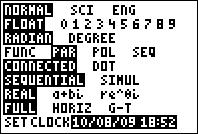
\includegraphics[width=2in]{./ParametricEquationsGraphics/Parametric01.jpg} &
\hspace{0.75in} 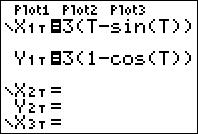
\includegraphics[width=2in]{./ParametricEquationsGraphics/Parametric02.jpg} \\

\end{tabular} 

\end{center}

Our next step is to find appropriate bounds on the parameter, $t$, as well as for $x$ and $y$.   We know that one full revolution of the circle occurs over the interval $0 \leq t < 2\pi$, so it seems reasonable to keep these as our bounds on $t$.  The `Tstep' seems reasonably small -- too large a value here can lead to incorrect graphs.\footnote{Again, see page \pageref{polargraphscalculator} in Section \ref{PolarGraphs}.}  We know from our derivation of the equations of the cycloid that the center of the generating circle has coordinates $(r\theta,r)  = (3t,3)$.  Since  $t$ ranges between $0$ and $2\pi$, we set $x$ to range between $0$ and $6\pi$.  The values of $y$ go from the bottom of the circle to the top, so $y$ ranges between $0$ and $6$.

\begin{center}
\begin{tabular}{cc}

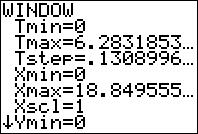
\includegraphics[width=2in]{./ParametricEquationsGraphics/Parametric03.jpg} &
\hspace{0.75in} 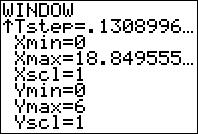
\includegraphics[width=2in]{./ParametricEquationsGraphics/Parametric04.jpg} \\

\end{tabular} 


\end{center}

Below we graph the cycloid with these settings, and then extend $t$ to range from $0$ to $6\pi$ which forces $x$ to range from $0$ to $18\pi$ yielding three arches of the cycloid.\footnote{It is instructive to note that keeping the $y$ settings between 0 and 6 skews the aspect ratio of the cycloid.  Using the `Zoom Square' feature on the graphing calculator gives a true geometric perspective of the three arches.}

\begin{center}

\begin{tabular}{cc}

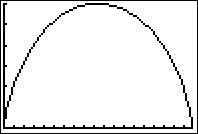
\includegraphics[width=2in]{./ParametricEquationsGraphics/Parametric05.jpg} &
\hspace{0.75in} 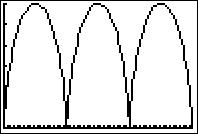
\includegraphics[width=2in]{./ParametricEquationsGraphics/Parametric06.jpg} \\


\end{tabular} 
\end{center}


In Exercises \ref{paracalcfirst} - \ref{paracalclast}, plot the set of parametric equations with the help of a graphing utility.  Be sure to indicate the orientation imparted on the curve by the parametrization.  

\begin{multicols}{2} \raggedcolumns 
\begin{enumerate}
\setcounter{enumi}{\value{HW}}


\item ${\displaystyle \left\{ \begin{array}{l} x = t^{3} - 3t \\ y = t^{2} - 4 \end{array} \right. \vspace{.25in} \mbox{for } -2 \leq t \leq 2}$ \label{paracalcfirst}
\item ${\displaystyle \left\{ \begin{array}{l} x = 4\cos^{3}(t) \\ y = 4\sin^{3}(t) \end{array} \right. \vspace{.25in} \mbox{for } 0 \leq t \leq 2\pi}$

\setcounter{HW}{\value{enumi}}
\end{enumerate}
\end{multicols}

\begin{multicols}{2} \raggedcolumns 
\begin{enumerate}
\setcounter{enumi}{\value{HW}}


\item ${\displaystyle \left\{ \begin{array}{l} x = e^{t} + e^{-t} \\ y = e^{t} - e^{-t} \end{array} \right. \vspace{.25in} \mbox{for }  -2 \leq t \leq 2}$
\item ${\displaystyle \left\{ \begin{array}{l} x = \cos(3t) \\ y = \sin(4t) \end{array} \right. \vspace{.25in} \mbox{for } 0 \leq t \leq 2\pi}$ \label{paracalclast}

\setcounter{HW}{\value{enumi}}
\end{enumerate}
\end{multicols}


In Exercises \ref{findparamfirst} - \ref{findparamlast}, find a parametric description for the given oriented curve.

\begin{enumerate}

\setcounter{enumi}{\value{HW}}

\item  the directed line segment from $(3,-5)$ to $(-2,2)$ \label{findparamfirst}

\item  the directed line segment from $(-2,-1)$ to $(3, -4)$ 

\item  the curve $y = 4-x^2$ from $(-2,0)$ to $(2,0)$.

\item   the curve $y = 4-x^2$ from $(-2,0)$ to $(2,0)$ \\
(Shift the parameter so  $t=0$ corresponds to $(-2,0)$.)

\item  the curve $x = y^2 - 9$ from $(-5,-2)$ to $(0,3)$.

\item  the curve $x = y^2 - 9$ from $(0,3)$ to $(-5,-2)$.\\
(Shift the parameter so  $t=0$ corresponds to $(0,3)$.)

\item   the circle $x^2 + y^2 = 25$, oriented counter-clockwise

\item   the circle $(x-1)^2 + y^2 = 4$, oriented counter-clockwise

\item   the circle $x^2 + y^2 - 6y = 0$, oriented counter-clockwise

\item   the circle $x^2 + y^2 - 6y = 0$, oriented \emph{clockwise}\\
(Shift the parameter so  $t$ begins at $0$.)

\item   the circle $(x-3)^2 + (y+1)^2 = 117$, oriented counter-clockwise

\item   the ellipse $(x-1)^2 + 9y^2 = 9$, oriented counter-clockwise

\item   the ellipse $9x^2 + 4y^2 + 24y =0$, oriented counter-clockwise

\item   the ellipse $9x^2 + 4y^2 + 24y =0$, oriented clockwise  \\
(Shift the parameter so $t=0$ corresponds to  $(0,0)$.)

\item  the triangle with vertices $(0,0)$, $(3,0)$, $(0,4)$, oriented counter-clockwise \\
(Shift the parameter so $t=0$ corresponds to $(0,0)$.) \label{findparamlast}

\setcounter{HW}{\value{enumi}}

\end{enumerate}

\begin{enumerate}

\setcounter{enumi}{\value{HW}}

\item Use parametric equations and a graphing utility to graph the inverse of $f(x) = x^{3} + 3x - 4$.

\item  Every polar curve $r = f(\theta)$ can be translated to a system of parametric equations with parameter $\theta$ by $\left\{ x = r\cos(\theta) = f(\theta) \cos(\theta), \, y = r \sin(\theta) = f(\theta) \sin(\theta) \right.$.  Convert $r = 6\cos(2\theta)$ to a system of parametric equations. Check your answer by graphing $r = 6\cos(2\theta)$ by hand using the techniques presented in Section \ref{PolarGraphs} and then graphing the parametric equations you found using a graphing utility.


\item  Use your results from Exercises \ref{heightlondoneye} and \ref{leftrightlondoneye} in Section \ref{Sinusoid} to find the parametric equations which model a passenger's position as they ride the \href{http://en.wikipedia.org/wiki/London_Eye}{\underline{London Eye}}. 




\setcounter{HW}{\value{enumi}}
\end{enumerate}

\phantomsection
\label{projectoilemotion}

Suppose an object, called a projectile, is launched into the air.  Ignoring everything except the force gravity, the path of the projectile is given by\footnote{A nice mix of vectors and Calculus are needed to derive this.}

\[ \left\{ \begin{array}{l} x =   v_{\text{\tiny $0$}} \cos(\theta) \, t \\ [3pt]
															y = -\dfrac{1}{2} g t^2 +  v_{\text{\tiny $0$}} \sin(\theta) \, t + s_{\text{\tiny $0$}} \\ \end{array} \right. \; \text{for} \; 0 \leq t \leq T \]

where  $v_{\text{\tiny $0$}}$ is the initial speed of the object, $\theta$ is the angle from the horizontal at which the projectile is launched,\footnote{We've seen this before.  It's the angle of elevation which was defined on page \pageref{angleofelevation}.} $g$ is the acceleration due to gravity,  $s_{\text{\tiny $0$}}$ is the initial height of the projectile above the ground and $T$ is the time when the object returns to the ground.  (See the figure below.)

\begin{center}

\begin{mfpic}[20]{-1}{9}{-1}{7}
\axes
\tlabel[cc](9,-0.5){\scriptsize $x$}
\tlabel[cc](0.5,7){\scriptsize $y$}
\dashed \polyline{(0,4), (1.5,4)}
\tlabelsep{5pt}
\axislabels{y}{{\scriptsize $s_{\text{\tiny $0$}}$} 4}
\point[4pt]{(0,4), (5.98,0)}
\arrow \shiftpath{(0,4)}  \parafcn{5, 55, 5}{0.75*dir(t)}
\tlabel[cc](1,4.5){\scriptsize $\theta$}
\tlabel[cc](5.98,-0.5){\scriptsize $(x(T), 0)$}
\penwd{1.25pt}
\arrow \parafcn{0,0.75,0.1}{(3.5*t, 6.062*t+4-(4.9*(t**2)))}
\parafcn{0.75,1.71,0.1}{(3.5*t, 6.062*t+4-(4.9*(t**2)))}

\end{mfpic}


\end{center}

\begin{enumerate}
\setcounter{enumi}{\value{HW}}

\item  Carl's friend Jason competes in Highland Games Competitions across the country.  In one event, the `hammer throw',  he throws a 56 pound weight for distance. If the weight is released $6$ feet above the ground at an angle of $42^{\circ}$ with respect to the horizontal with an initial speed of $33$ feet per second, find the parametric equations for the flight of the hammer.  (Here, use $g = 32 \frac{\text{ft.}}{s^2}$.) When will the hammer hit the ground?  How far away will it hit the ground? Check your answer using a graphing utility.

\item  \label{projectileeliminate} Eliminate the parameter in the equations for projectile motion to show that the path of the projectile follows the curve \[y = -\dfrac{g \sec^{2}(\theta)}{2 v_{\text{\tiny$0$}}^2} x^2 + \tan(\theta) x + s_{\text{\tiny $0$}}\] Use the vertex formula (Equation \ref{vertexofquadraticfunctions}) to show the maximum height of the projectile is \[y = \dfrac{v_{\text{\tiny$0$}}^2 \sin^{2}(\theta)}{2g} + s_{\text{\tiny $0$}} \quad \text{when} \quad x = \dfrac{v_{\text{\tiny$0$}}^2 \sin(2\theta) }{2g}\] 

\item  In another event, the `sheaf toss', Jason throws a  20 pound weight for height.  If the weight is released  5 feet above the ground at an angle of $85^{\circ}$ with respect to the horizontal and the sheaf reaches a maximum height of 31.5 feet, use your results from part  \ref{projectileeliminate} to determine how fast the sheaf was launched into the air.  (Once again, use $g = 32 \frac{\text{ft.}}{s^2}$.)

\item  Suppose $\theta = \frac{\pi}{2}$. (The projectile was launched vertically.) Simplify the general parametric formula given for $y(t)$ above using  $g = 9.8 \, \frac{m}{s^2}$ and compare that to the formula for $s(t)$ given in Exercise \ref{whatgoesup} in Section \ref{QuadraticFunctions}.  What is $x(t)$ in this case?

\item  If $f$ and $g$ are functions, explain why the function $\vec{r}(t) = \left<f(t), g(t) \right>$ is a function. The function $\vec{r}$ is called a \index{function ! vector-valued}\index{vector-valued function}\textbf{vector-valued function} since it matches real number inputs, $t$, with vector outputs, $\vec{r}(t)$.   Explain why when the vectors  $\vec{r}(t)$ are plotted in standard position, their terminal points trace out the curve described parametrically by the system of equations:  $\left\{ x = f(t) \, y =  g(t) \right.$  (In Calculus, you will see  systems of parametric equations `packaged' together using vectors.)

\setcounter{HW}{\value{enumi}}
\end{enumerate}


\phantomsection
\label{hyperboliccosinesine} 

In Exercises \ref{hyperbolicfirst} - \ref{hyperboliclast}, we explore the  \textbf{hyperbolic cosine}\index{hyperbolic cosine} function, denoted $\cosh(t)$, and the \textbf{hyperbolic sine}\index{hyperbolic sine}
function, denoted $\sinh(t)$, defined below:

\[ \begin{array}{ccc}

\cosh(t) = \dfrac{e^{t} + e^{-t}}{2} & 
\text{and} & \sinh(t) = \dfrac{e^{t} - e^{-t}}{2} \\

\end{array} \]

\begin{enumerate}
\setcounter{enumi}{\value{HW}}

\item  Using a graphing utility as needed, verify the following:  \label{hyperbolicfirst}

\begin{enumerate}

\item the domain of $\cosh(t)$ is $(-\infty, \infty)$ and the range of $\cosh(t)$ is $[1,\infty)$.

\item  the domain and range  of $\sinh(t)$ are both $(-\infty, \infty)$.

\end{enumerate}

\item  Show that $\left\{ x(t) = \cosh(t), \, y(t) = \sinh(t) \right.$ parametrize the right half of the `unit' hyperbola $x^2 - y^2 = 1$.  (Hence the use of the adjective `hyperbolic.')

\item  Compare and contrast the definitions of $\cosh(t)$ and $\sinh(t)$ to the formulas for $\cos(t)$ and $\sin(t)$ given in Exercise \ref{expformcosandsin} in Section \ref{PolarComplex}.

\item \label{andtheresthyperbolic} Four other hyperbolic functions are waiting to be defined:  the hyperbolic secant $\text{sech}(t)$, the hyperbolic cosecant $\text{csch}(t)$, the hyperbolic tangent $\tanh(t)$ and the hyperbolic cotangent $\coth(t)$.  Define these functions in terms of $\cosh(t)$ and $\sinh(t)$, then convert them to formulas involving $e^{t}$ and $e^{-t}$.  Consult a suitable reference (a Calculus book, or this entry on the \href{http://en.wikipedia.org/wiki/Hyperbolic_function}{\underline{hyperbolic functions}}) and spend some time reliving the thrills of trigonometry with these `hyperbolic' functions.

\item  If these functions look familiar, they should.  Enjoy some nostalgia and revisit Exercise \ref{catenary} in Section \ref{ExpLogApplications}, Exercise \ref{hyperbolicsine} in Section \ref{ExponentialEquationsandInequalities} and the  answer to Exercise \ref{inversehyptangent} in Section \ref{LogarithmicEquationsandInequalities}. \label{hyperboliclast}

\end{enumerate}

\newpage

\subsection{Answers}

\begin{multicols}{2} \raggedcolumns 
\begin{enumerate}

\item ${\displaystyle \left\{ \begin{array}{l} x = 4t-3 \\ y = 6t-2 \end{array} \right. \vspace{.25in} \mbox{for } 0 \leq t \leq 1}$

\begin{mfpic}[15]{-4}{2}{-3}{5}
\axes
\tlabel[cc](2,-0.5){\scriptsize $x$}
\tlabel[cc](0.5,5){\scriptsize $y$}
\xmarks{-3,-2,-1,1}
\ymarks{-2,-1,1,2,3,4}
\point[4pt]{(-3,-2), (1,4)}
\tlpointsep{4pt}
\scriptsize
\axislabels {x}{{$-3 \hspace{6pt}$} -3,{$-2 \hspace{6pt}$} -2,{$-1 \hspace{6pt}$} -1, {$1$} 1}
\axislabels {y}{{$-1$} -1,{$-2$} -2, {$1$} 1,{$2$} 2,{$3$} 3,{$4$} 4}
\normalsize
\penwd{1.25pt}
\arrow \parafcn{0,0.5,0.1}{(4*t-3,6*t-2)}
\parafcn{0.5,1,0.1}{(4*t-3,6*t-2)}
\end{mfpic}


\item ${\displaystyle \left\{ \begin{array}{l} x = 4t-1 \\ y = 3-4t \end{array} \right. \vspace{.25in} \mbox{for } 0 \leq t \leq 1}$


\begin{mfpic}[15]{-2}{4}{-2}{4}
\axes
\tlabel[cc](4,-0.5){\scriptsize $x$}
\tlabel[cc](0.5,4){\scriptsize $y$}
\xmarks{-1,1,2,3}
\ymarks{-1,1,2,3}
\point[4pt]{(-1,3), (3,-1)}
\tlpointsep{4pt}
\scriptsize
\axislabels {x}{{$-1 \hspace{6pt}$} -1, {$1$} 1, {$2$} 2,{$3$} 3}
\axislabels {y}{{$-1$} -1, {$1$} 1,{$2$} 2,{$3$} 3}
\normalsize
\penwd{1.25pt}
\arrow \parafcn{0,0.5,0.1}{(4*t-1,3-4*t)}
\parafcn{0.5,1,0.1}{(4*t-1,3-4*t)}
\end{mfpic}
\setcounter{HW}{\value{enumi}}
\end{enumerate}
\end{multicols}



\begin{multicols}{2} \raggedcolumns 
\begin{enumerate}
\setcounter{enumi}{\value{HW}}

\item ${\displaystyle \left\{ \begin{array}{l} x = 2t \\ y = t^2 \end{array} \right. \vspace{.25in} \mbox{for } -1 \leq t \leq 2}$

\begin{mfpic}[15]{-3}{5}{-1}{5}
\axes
\tlabel[cc](5,-0.5){\scriptsize $x$}
\tlabel[cc](0.5,5){\scriptsize $y$}
\xmarks{-2,-1,1,2,3,4}
\ymarks{1,2,3,4}
\point[4pt]{(-2,1), (0,0), (4,4)}
\tlpointsep{4pt}
\scriptsize
\axislabels {x}{{$-3 \hspace{6pt}$} -3,{$-2 \hspace{6pt}$} -2,{$-1 \hspace{6pt}$} -1, {$1$} 1, {$2$} 2,{$3$} 3,{$4$} 4}
\axislabels {y}{{$1$} 1,{$2$} 2,{$3$} 3,{$4$} 4}
\normalsize
\penwd{1.25pt}
\arrow \parafcn{-1,-0.5,0.1}{(2*t,(t**2))}
\arrow \parafcn{-0.5,1,0.1}{(2*t,(t**2))}
\parafcn{1,2,0.1}{(2t,t**2)}
\end{mfpic}


\item ${\displaystyle \left\{ \begin{array}{l} x = t-1 \\ y = 3+2t-t^2 \end{array} \right. \vspace{.25in} \mbox{for } 0 \leq t \leq 3}$


\begin{mfpic}[15]{-2}{3}{-1}{5}
\axes
\tlabel[cc](4,-0.5){\scriptsize $x$}
\tlabel[cc](0.5,5){\scriptsize $y$}
\xmarks{-1,1,2}
\ymarks{1,2,3,4}
\point[4pt]{(-1,3), (0,4), (2,0)}
\tlpointsep{4pt}
\scriptsize
\axislabels {x}{{$-1 \hspace{6pt}$} -1, {$1$} 1, {$2$} 2}
\axislabels {y}{{$1$} 1,{$2$} 2,{$3$} 3,{$4$} 4}
\normalsize
\penwd{1.25pt}
\arrow \parafcn{0,0.5,0.1}{(t-1,3+2*t-(t**2))}
\arrow \parafcn{0.5,2,0.1}{(t-1,3+2*t-(t**2))}
\parafcn{2,3,0.1}{(t-1,3+2*t-(t**2))}

\end{mfpic}

\setcounter{HW}{\value{enumi}}
\end{enumerate}
\end{multicols}


\begin{multicols}{2} \raggedcolumns 
\begin{enumerate}
\setcounter{enumi}{\value{HW}}

\item ${\displaystyle \left\{ \begin{array}{l} x = t^2+2t+1 \\ y = t+1 \end{array} \right. \vspace{.25in} \mbox{for } t \leq 1}$

\begin{mfpic}[15]{-1}{6}{-3}{3}
\axes
\tlabel[cc](6,-0.5){\scriptsize $x$}
\tlabel[cc](0.5,3){\scriptsize $y$}
\xmarks{1,2,3,4,5}
\ymarks{-2,-1,1,2}
\point[4pt]{(4,2), (0,0), (4,-2)}
\tlpointsep{4pt}
\scriptsize
\axislabels {x}{ {$1$} 1, {$2$} 2,{$3$} 3,{$4$} 4,{$5$} 5}
\axislabels {y}{{$-2$} -2,{$-1$} -1,{$1$} 1,{$2$} 2,{$3$}}
\normalsize
\penwd{1.25pt}
\parafcn{0,1,0.1}{((t**2)+(2*t)+1,t+1)}
\arrow \parafcn{-2,0,0.1}{((t**2)+(2*t)+1,t+1)}
\arrow \parafcn{-3.25,-2,0.1}{((t**2)+(2*t)+1,t+1)}
\arrow \parafcn{-3.44,-3.25,0.1}{((t**2)+(2*t)+1,t+1)}
\end{mfpic} 

\item ${\displaystyle \left\{ \begin{array}{l} x = \frac{1}{9}\left(18-t^2\right) \\ y = \frac{1}{3} t \end{array} \right. \vspace{.25in} \mbox{for } t \geq -3}$



\begin{mfpic}[15]{-4}{3}{-2}{3}
\axes
\tlabel[cc](3,-0.5){\scriptsize $x$}
\tlabel[cc](0.5,3){\scriptsize $y$}
\xmarks{-3,-2,-1,1,2}
\ymarks{-1,1,2}
\point[4pt]{(1,-1), (2,0), (-2,2)}
\tlpointsep{4pt}
\scriptsize
\axislabels {x}{{$-3 \hspace{6pt}$} -3,{$-2 \hspace{6pt}$} -2,{$-1 \hspace{6pt}$} -1, {$1$} 1, {$2$} 2}
\axislabels {y}{{$-1$} -1,{$1$} 1,{$2$} 2}
\normalsize
\penwd{1.25pt}
\arrow \parafcn{-3,-1.5,0.1}{((18-(t**2))/9,t/3)}
\arrow \parafcn{-1.5,3,0.1}{((18-(t**2))/9,t/3)}
\arrow \parafcn{3,6.5,0.1}{((18-(t**2))/9,t/3)}

\end{mfpic}

\setcounter{HW}{\value{enumi}}
\end{enumerate}
\end{multicols}


\pagebreak


\begin{multicols}{2} \raggedcolumns 
\begin{enumerate}
\setcounter{enumi}{\value{HW}}

\item ${\displaystyle \left\{ \begin{array}{l} x = t \\ y = t^3 \end{array} \right. \vspace{.25in} \mbox{for } -\infty < t < \infty}$


\begin{mfpic}[15]{-2}{2}{-5}{5}
\axes
\tlabel[cc](2,-0.5){\scriptsize $x$}
\tlabel[cc](0.5,5){\scriptsize $y$}
\xmarks{-1,1}
\ymarks{-4,-3,-2,-1,1,2,3,4}
\point[4pt]{(-1,-1), (0,0), (1,1)}
\tlpointsep{4pt}
\scriptsize
\axislabels {x}{{$-1 \hspace{6pt}$} -1, {$1$} 1}
\axislabels {y}{{$-4$} -4,{$-3$} -3,{$-2$} -2,{$-1$} -1,{$1$} 1,{$2$} 2,{$3$} 3,{$4$} 4}
\normalsize
\penwd{1.25pt}
\arrow \parafcn{-1.7,-1.25,0.1}{(t, t**3)}
\arrow \parafcn{-1.25,1.25,0.1}{(t, t**3)}
\arrow \parafcn{1.25,1.7,0.1}{(t, t**3)}
\end{mfpic}


\item ${\displaystyle \left\{ \begin{array}{l} x = t^3 \\ y = t \end{array} \right. \vspace{.25in} \mbox{for } -\infty < t < \infty}$

\begin{mfpic}[15]{-5}{5}{-2}{2}
\axes
\tlabel[cc](5,-0.5){\scriptsize $x$}
\tlabel[cc](0.5,2){\scriptsize $y$}
\xmarks{-4,-3,-2,-1,1,2,3,4}
\ymarks{-1,1}
\point[4pt]{(-1,-1), (0,0), (1,1)}
\tlpointsep{4pt}
\scriptsize
\axislabels {y}{{$-1$} -1, {$1$} 1}
\axislabels {x}{{$-4 \hspace{6pt}$} -4,{$-3 \hspace{6pt}$} -3,{$-2 \hspace{6pt}$} -2,{$-1 \hspace{6pt}$} -1,{$1$} 1,{$2$} 2,{$3$} 3,{$4$} 4}
\normalsize
\penwd{1.25pt}
\arrow \parafcn{-1.7,-1.25,0.1}{(t**3, t)}
\arrow \parafcn{-1.25,1.25,0.1}{(t**3, t)}
\arrow \parafcn{1.25,1.7,0.1}{(t**3, t)}
\end{mfpic}


\setcounter{HW}{\value{enumi}}
\end{enumerate}
\end{multicols}



\begin{multicols}{2}

\begin{enumerate}

\setcounter{enumi}{\value{HW}}
\item ${\displaystyle \left\{ \begin{array}{l} x = \cos(t) \\ y = \sin(t) \end{array} \right. \vspace{.25in} \mbox{for } -\dfrac{\pi}{2} \leq t \leq \dfrac{\pi}{2}}$

\begin{mfpic}[10]{-5}{5}{-5}{5}
\axes
\tlabel[cc](5,-0.5){\scriptsize $x$}
\tlabel[cc](0.5,5){\scriptsize $y$}
\point[4pt]{(0,-4), (4,0), (0,4)}
\xmarks{-4,4}
\ymarks{-4,4}
\tlpointsep{4pt}
\scriptsize
\axislabels {x}{{$-1 \hspace{6pt}$} -4, {$1$} 4}
\axislabels {y}{{$-1$} -4, {$1$} 4}
\normalsize
\penwd{1.25pt}
\arrow \parafcn{-1.57,-0.78,0.1}{(4*cos(t),4*sin(t))}
\arrow \parafcn{-0.78,0.78,0.1}{(4*cos(t),4*sin(t))}
\parafcn{0.78,1.57,0.1}{(4*cos(t),4*sin(t))}
\end{mfpic} 


\item ${\displaystyle \left\{ \begin{array}{l} x = 3\cos(t) \\ y = 3\sin(t) \end{array} \right. \vspace{.25in} \mbox{for } 0 \leq t \leq \pi}$

\begin{mfpic}[15]{-4}{4}{-1}{4}
\axes
\tlabel[cc](4,-0.5){\scriptsize $x$}
\tlabel[cc](0.5,4){\scriptsize $y$}
\point[4pt]{(-3,0), (3,0), (0,3)}
\xmarks{-3,-2,-1,1,2,3}
\ymarks{1,2,3}
\tlpointsep{4pt}
\scriptsize
\axislabels {x}{{$-3 \hspace{6pt}$} -3, {$-2 \hspace{6pt}$} -2,{$-1 \hspace{6pt}$} -1,{$1$} 1,{$2$} 2,{$3$} 3}
\axislabels {y}{{$1$} 1,{$2$} 2,{$3$} 3}
\normalsize
\penwd{1.25pt}
\arrow \parafcn{0,0.78,0.1}{(3*cos(t),3*sin(t))}
\arrow \parafcn{0.78,2.36,0.1}{(3*cos(t),3*sin(t))}
\parafcn{2.36,3.14,0.1}{(3*cos(t),3*sin(t))}
\end{mfpic} 

\setcounter{HW}{\value{enumi}}
\end{enumerate}
\end{multicols}




\begin{multicols}{2}
\begin{enumerate}
\setcounter{enumi}{\value{HW}}

\item  ${\displaystyle \left\{ \begin{array}{l} x = -1+3\cos(t) \\ y = 4\sin(t) \end{array} \right. \vspace{.25in} \mbox{for } 0 \leq t \leq 2\pi}$

\begin{mfpic}[15]{-5}{3}{-5}{5}
\axes
\tlabel[cc](3,-0.5){\scriptsize $x$}
\tlabel[cc](0.5,5){\scriptsize $y$}
\point[4pt]{(2,0), (-1,4), (-4,0), (-1,-4)}
\xmarks{-4,-3,-2,-1,1,2}
\ymarks{-4,-3,-2,-1,1,2,3,4}
\tlpointsep{4pt}
\scriptsize
\axislabels {x}{{$-4 \hspace{6pt}$} -4,{$-3 \hspace{6pt}$} -3,{$-2 \hspace{6pt}$} -2, {$-1 \hspace{6pt}$} -1,{$1$} 1,{$2$} 2}
\axislabels {y}{{$-4$} -4, {$-3$} -3,{$-2$} -2,{$-1$} -1,{$1$} 1,{$2$} 2,{$3$} 3,{$4$} 4}
\normalsize
\penwd{1.25pt}
\arrow \parafcn{0,0.78,0.1}{(3*cos(t)-1,4*sin(t))}
\arrow \parafcn{0.78,2.36, 0.1}{(3*cos(t)-1,4*sin(t))}
\arrow \parafcn{2.36,3.93, 0.1}{(3*cos(t)-1,4*sin(t))}
\arrow \parafcn{3.93,5.5, 0.1}{(3*cos(t)-1,4*sin(t))}
\parafcn{5.5,6.28, 0.1}{(3*cos(t)-1,4*sin(t))}
\end{mfpic} 

\item ${\displaystyle \left\{ \begin{array}{l} x = 3\cos(t) \\ y = 2\sin(t)+1 \end{array} \right. \vspace{.25in} \mbox{for } \dfrac{\pi}{2} \leq t \leq 2\pi}$

\begin{mfpic}[15]{-4}{4}{-2}{4}
\axes
\tlabel[cc](4,-0.5){\scriptsize $x$}
\tlabel[cc](0.5,4){\scriptsize $y$}
\point[4pt]{(0,3), (-3,1), (0,-1), (3,1)}
\xmarks{-3,-2,-1,1,2,3}
\ymarks{-1,1,2,3}
\tlpointsep{4pt}
\scriptsize
\axislabels {x}{{$-3 \hspace{6pt}$} -3, {$-1 \hspace{6pt}$} -1,{$1$} 1,{$3$} 3}
\axislabels {y}{{$-1$} -1,{$1$} 1,{$2$} 2,{$3$} 3}
\normalsize
\penwd{1.25pt}
\arrow \parafcn{1.57,2.36,0.1}{(3*cos(t),1+2*sin(t))}
\arrow \parafcn{2.36,3.93,0.1}{(3*cos(t),1+2*sin(t))}
\arrow \parafcn{3.93,5.50,0.1}{(3*cos(t),1+2*sin(t))}
\parafcn{5.50,6.28,0.1}{(3*cos(t),1+2*sin(t))}
\end{mfpic} 

\setcounter{HW}{\value{enumi}}
\end{enumerate}
\end{multicols}

\begin{multicols}{2} \raggedcolumns 
\begin{enumerate}
\setcounter{enumi}{\value{HW}}

\item ${\displaystyle \left\{ \begin{array}{l} x = 2\cos(t) \\ y = \sec(t) \end{array} \right. \vspace{.25in} \mbox{for } 0 \leq t < \dfrac{\pi}{2}}$


\begin{mfpic}[25]{-1}{5}{-1}{5}
\axes
\tlabel[cc](5,-0.5){\scriptsize $x$}
\tlabel[cc](0.5,5){\scriptsize $y$}
\point[4pt]{(2,1)}
\xmarks{1,2,3,4}
\ymarks{1,2,3,4}
\tlpointsep{4pt}
\scriptsize
\axislabels {x}{{$1$} 1,{$2$} 2,{$3$} 3,{$4$} 4}
\axislabels {y}{{$1$} 1,{$2$} 2,{$3$} 3,{$4$} 4}
\normalsize
\penwd{1.25pt}
\arrow \parafcn{0,1,0.1}{(2*cos(t),sec(t))}
\arrow \parafcn{1,1.31,0.1}{(2*cos(t),sec(t))}
\end{mfpic} 


\item ${\displaystyle \left\{ \begin{array}{l} x = 2\tan(t) \\ y = \cot(t) \end{array} \right. \vspace{.25in} \mbox{for } 0 < t < \dfrac{\pi}{2}}$

\begin{mfpic}[25]{-1}{5}{-1}{5}
\axes
\tlabel[cc](5,-0.5){\scriptsize $x$}
\tlabel[cc](0.5,5){\scriptsize $y$}

\xmarks{1,2,3,4}
\ymarks{1,2,3,4}
\tlpointsep{4pt}
\scriptsize
\axislabels {x}{{$1$} 1,{$2$} 2,{$3$} 3,{$4$} 4}
\axislabels {y}{{$1$} 1,{$2$} 2,{$3$} 3,{$4$} 4}
\normalsize
\penwd{1.25pt}
\arrow \parafcn{0.25,0.4,0.1}{(2*tan(t),cot(t))}
\arrow \parafcn{0.4,0.7,0.1}{(2*tan(t),cot(t))}
\arrow \parafcn{0.7,1.1,0.1}{(2*tan(t),cot(t))}
\end{mfpic} 

\setcounter{HW}{\value{enumi}}
\end{enumerate}
\end{multicols}





\begin{multicols}{2}
\begin{enumerate}
\setcounter{enumi}{\value{HW}}

\item ${\displaystyle \left\{ \begin{array}{l} x = \sec(t) \\ y = \tan(t) \end{array} \right. \vspace{.25in} \mbox{for } -\dfrac{\pi}{2} < t < \dfrac{\pi}{2}}$

\begin{mfpic}[15]{-1}{5}{-5}{5}
\axes
\tlabel[cc](5,-0.5){\scriptsize $x$}
\tlabel[cc](0.5,5){\scriptsize $y$}
\point[4pt]{(1,0)}
\xmarks{1,2,3,4}
\ymarks{-4,-3,-2,-1,1,2,3,4}
\tlpointsep{4pt}
\scriptsize
\axislabels {x}{{$1$} 1,{$2$} 2,{$3$} 3,{$4$} 4}
\axislabels {y}{{$-4$} -4, {$-3$} -3,{$-2$} -2,{$-1$} -1,{$1$} 1,{$2$} 2,{$3$} 3,{$4$} 4}
\normalsize
\dashed \polyline{(4,4),(-1,-1)}
\dashed \polyline{(4,-4),(-1,1)}
\penwd{1.25pt}
\arrow \parafcn{1.85,2,0.1}{(0-sec(t),tan(t))}
\arrow \parafcn{2,4.25,0.1}{(0-sec(t),tan(t))}
\arrow \parafcn{4.25,4.4,0.1}{(0-sec(t),tan(t))}

\end{mfpic} 

\item ${\displaystyle \left\{ \begin{array}{l} x = \sec(t) \\ y = \tan(t) \end{array} \right. \vspace{.25in} \mbox{for } \dfrac{\pi}{2} < t < \dfrac{3\pi}{2}}$

\begin{mfpic}[15]{-5}{1}{-5}{5}
\axes
\tlabel[cc](1,-0.5){\scriptsize $x$}
\tlabel[cc](0.5,5){\scriptsize $y$}
\point[4pt]{(-1,0)}
\xmarks{-4,-3,-2,-1}
\ymarks{-4,-3,-2,-1,1,2,3,4}
\tlpointsep{4pt}
\scriptsize
\axislabels {x}{{$-4 \hspace{6pt}$} -4,{$-3 \hspace{6pt}$} -3,{$-2 \hspace{6pt}$} -2, {$-1 \hspace{6pt}$} -1}
\axislabels {y}{{$-4$} -4, {$-3$} -3,{$-2$} -2,{$-1$} -1,{$1$} 1,{$2$} 2,{$3$} 3,{$4$} 4}
\normalsize
\dashed \polyline{(-4,4),(1,-1)}
\dashed \polyline{(-4,-4),(1,1)}
\penwd{1.25pt}
\arrow \parafcn{1.85,2,0.1}{(sec(t),tan(t))}
\arrow \parafcn{2,4.25,0.1}{(sec(t),tan(t))}
\arrow \parafcn{4.25,4.4,0.1}{(sec(t),tan(t))}

\end{mfpic} 

\setcounter{HW}{\value{enumi}}
\end{enumerate}

\end{multicols}


\pagebreak

\begin{multicols}{2}
\begin{enumerate}
\setcounter{enumi}{\value{HW}}

\item ${\displaystyle \left\{ \begin{array}{l} x = \tan(t) \\ y = 2\sec(t) \end{array} \right. \vspace{.25in} \mbox{for } -\dfrac{\pi}{2} < t < \dfrac{\pi}{2}}$

\begin{mfpic}[25]{-3}{3}{-1}{5}
\axes
\tlabel[cc](3,-0.5){\scriptsize $x$}
\tlabel[cc](0.5,5){\scriptsize $y$}
\point[4pt]{(0,2)}
\xmarks{-2,-1,1,2}
\ymarks{1,2,3,4}
\tlpointsep{4pt}
\scriptsize
\axislabels {x}{{$-2 \hspace{6pt}$} -2,{$-1 \hspace{6pt}$} -1, {$1$} 1,{$2$} 2}
\axislabels {y}{{$1$} 1,{$2$} 2,{$3$} 3,{$4$} 4}
\normalsize
\dashed \polyline{(-0.5,-1),(2,4)}
\dashed \polyline{(0.5,-1),(-2,4)}
\penwd{1.25pt}
\arrow \parafcn{-1,-0.75,0.1}{(tan(t),2*sec(t))}
\arrow \parafcn{-0.75,1,0.1}{(tan(t),2*sec(t))}
\end{mfpic} 

\item ${\displaystyle \left\{ \begin{array}{l} x = \tan(t) \\ y = 2\sec(t) \end{array} \right. \vspace{.25in} \mbox{for } \dfrac{\pi}{2} < t < \dfrac{3\pi}{2}}$


\begin{mfpic}[25]{-3}{3}{-5}{1}
\axes
\tlabel[cc](3,-0.5){\scriptsize $x$}
\tlabel[cc](0.5,1){\scriptsize $y$}
\point[4pt]{(0,-2)}
\xmarks{-2,-1,1,2}
\ymarks{-1,-2,-3,-4}
\tlpointsep{4pt}
\scriptsize
\axislabels {x}{{$-2 \hspace{6pt}$} -2,{$-1 \hspace{6pt}$} -1, {$1$} 1,{$2$} 2}
\axislabels {y}{{$-1$} -1,{$-2$} -2,{$-3$} -3,{$-4$} -4}
\normalsize
\dashed \polyline{(-0.5,1),(2,-4)}
\dashed \polyline{(0.5,1),(-2,-4)}
\penwd{1.25pt}
\arrow \parafcn{-1,-0.75,0.1}{(tan(t),0-2*sec(t))}
\arrow \parafcn{-0.75,1,0.1}{(tan(t),0-2*sec(t))}
\end{mfpic} 
\setcounter{HW}{\value{enumi}}
\end{enumerate}

\end{multicols}

\begin{multicols}{2} \raggedcolumns 
\begin{enumerate}
\setcounter{enumi}{\value{HW}}

\item ${\displaystyle \left\{ \begin{array}{l} x = \cos(t) \\ y = t \end{array} \right. \vspace{.25in} \mbox{for } 0 < t < \pi}$

\begin{mfpic}[25]{-2.25}{2.25}{-0.5}{4}
\point[4pt]{(1,0), (0,1.5708), (-1,3.1416)}
\axes
\tlabel[cc](2.25,-0.25){\scriptsize $x$}
\tlabel[cc](0.25,4){\scriptsize $y$}

\xmarks{-1,1}
\ymarks{1.5708, 3.1416}
\tlpointsep{4pt}
\axislabels {y}{{\scriptsize $\frac{\pi}{2}$} 1.5708,  {\scriptsize $\pi$} 3.1416}
\axislabels {x}{{\scriptsize $-1 \hspace{7pt}$} -1, {\scriptsize $1$} 1}
\penwd{1.25pt}
\arrow \parafcn{0, 0.78, 0.1}{(cos(t), t)}
\arrow \parafcn{0.78, 2.36, 0.1}{(cos(t), t)}
\parafcn{2.36, 3.14, 0.1}{(cos(t), t)}

\end{mfpic}


\item ${\displaystyle \left\{ \begin{array}{l} x = \sin(t) \\ y = t \end{array} \right. \vspace{.25in} \mbox{for } -\dfrac{\pi}{2} < t < \dfrac{\pi}{2}}$

\begin{mfpic}[25]{-2}{2}{-2}{2}
\point[4pt]{(-1,-1.5708), (0,0), (1,1.5708)}
\axes
\tlabel[cc](2,-0.25){\scriptsize $x$}
\tlabel[cc](0.25,2){\scriptsize $y$}
\ymarks{-1.5708, 1.5708}
\xmarks{-1,1}
\tlpointsep{4pt}
\axislabels {y}{{\scriptsize $-\frac{\pi}{2}$} -1.5708, {\scriptsize $\frac{\pi}{2}$} 1.5708}
\axislabels {x}{{\scriptsize $-1 \hspace{7pt}$} -1, {\scriptsize $1$} 1}
\penwd{1.25pt}
\arrow \parafcn{-1.57, -0.78, 0.1}{(sin(t),t)}
\arrow \parafcn{-0.78,0.78, 0.1}{(sin(t),t)}
\arrow \parafcn{0.78, 1.57, 0.1}{(sin(t),t)}
\end{mfpic}


\setcounter{HW}{\value{enumi}}
\end{enumerate}
\end{multicols}


\begin{multicols}{2}
\begin{enumerate}
\setcounter{enumi}{\value{HW}}

\item ${\displaystyle \left\{ \begin{array}{l} x = t^{3} - 3t \\ y = t^{2} - 4 \end{array} \right. \vspace{.25in} \mbox{for } -2 \leq t \leq 2}$

\begin{mfpic}[15]{-3}{3}{-5}{1}
\axes
\tlabel[cc](3,-0.5){\scriptsize $x$}
\tlabel[cc](0.5,1){\scriptsize $y$}
\point[4pt]{(-2,0), (2,0), (0,-1), (0,-4)}
\xmarks{-2,-1,1,2}
\ymarks{-4,-3,-2,-1}
\tlpointsep{4pt}
\scriptsize
\axislabels {x}{{$-2 \hspace{6pt}$} -2, {$-1 \hspace{6pt}$} -1,{$1$} 1, {$2$} 2}
\axislabels {y}{{$-4$} -4, {$-3$} -3,{$-2$} -2,{$-1$} -1}
\normalsize
\penwd{1.25pt}
\arrow \parafcn{-2,-1,0.1}{(t**3 - 3*t,t**2 - 4)}
\arrow \parafcn{-1,1,0.1}{(t**3 - 3*t,t**2 - 4)}
\parafcn{1,2,0.1}{(t**3 - 3*t,t**2 - 4)}


\end{mfpic} 

\vspace{1in}

\item ${\displaystyle \left\{ \begin{array}{l} x = 4\cos^{3}(t) \\ y = 4\sin^{3}(t) \end{array} \right. \vspace{.25in} \mbox{for } 0 \leq t \leq 2\pi}$

\begin{mfpic}[12]{-5}{5}{-5}{5}
\axes
\tlabel[cc](5,-0.5){\scriptsize $x$}
\tlabel[cc](0.5,5){\scriptsize $y$}
\point[4pt]{(-4,0), (0,4), (4,0), (0,-4)}
\xmarks{-4,-3,-2,-1,1,2,3,4}
\ymarks{-4,-3,-2,-1,1,2,3,4}
\tlpointsep{4pt}
\scriptsize
\axislabels {x}{{$-4 \hspace{6pt}$} -4, {$-3 \hspace{6pt}$} -3,{$-2 \hspace{6pt}$} -2,{$-1 \hspace{6pt}$} -1,{$1$} 1, {$2$} 2, {$3$} 3, {$4$} 4}
\axislabels {y}{{$-4$} -4,{$-3$} -3,{$-2$} -2,{$-1$} -1,{$1$} 1,{$2$} 2,{$3$} 3, {$4$} 4}
\normalsize
\penwd{1.25pt}
\arrow \parafcn{0,0.78,0.1}{(4*((cos(t))**3),4*((sin(t))**3))}
\arrow \parafcn{0.78, 2.36,0.1}{(4*((cos(t))**3),4*((sin(t))**3))}
\arrow \parafcn{2.36, 3.93 ,0.1}{(4*((cos(t))**3),4*((sin(t))**3))}
\arrow \parafcn{3.93, 5.5 ,0.1}{(4*((cos(t))**3),4*((sin(t))**3))}
\parafcn{5.5, 6.28 ,0.1}{(4*((cos(t))**3),4*((sin(t))**3))}
\end{mfpic} 

\setcounter{HW}{\value{enumi}}

\end{enumerate}

\end{multicols}

\pagebreak

\begin{multicols}{2}

\begin{enumerate}
\setcounter{enumi}{\value{HW}}


\item ${\displaystyle \left\{ \begin{array}{l} x = e^{t} + e^{-t} \\ y = e^{t} - e^{-t} \end{array} \right. \vspace{.25in} \mbox{for }  -2 \leq t \leq 2}$

\begin{mfpic}[15][8.5]{-1}{8}{-8}{8}
\axes
\tlabel[cc](8,-0.5){\scriptsize $x$}
\tlabel[cc](0.5,8){\scriptsize $y$}
\point{(2,0), (7.52, 7.25), (7.52, -7.25)}
\xmarks{1,2,3,4,5,6,7}
\ymarks{-7,-6,-5,-4,-3,-2,-1,1,2,3,4,5,6,7}
\tlpointsep{4pt}
\scriptsize
\axislabels {x}{{$1$} 1, {$2$} 2, {$3$} 3,{$4$} 4,{$5$} 5,{$6$} 6, {$7$} 7}
\axislabels {y}{{$-7$} -7,{$-5$} -5,{$-3$} -3,{$-1$} -1, {$1$} 1, {$3$} 3, {$5$} 5, {$7$} 7}
\normalsize
\penwd{1.25pt}
\arrow \parafcn{-2,-1.5,0.1}{(exp(t) + exp(-t),exp(t) - exp(-t))}
\arrow \parafcn{-1.5,1.5,0.1}{(exp(t) + exp(-t),exp(t) - exp(-t))}
 \parafcn{1.5,2,0.1}{(exp(t) + exp(-t),exp(t) - exp(-t))}



\end{mfpic} 


\item ${\displaystyle \left\{ \begin{array}{l} x = \cos(3t) \\ y = \sin(4t) \end{array} \right. \vspace{.25in} \mbox{for } 0 \leq t \leq 2\pi}$

\begin{mfpic}[15]{-5}{5}{-5}{5}
\axes
\tlabel[cc](5,-0.5){\scriptsize $x$}
\tlabel[cc](0.5,5){\scriptsize $y$}
\xmarks{-4,4}
\ymarks{-4,4}
\tlpointsep{4pt}
\scriptsize
\axislabels {x}{{$-1 \hspace{6pt}$} -4, {$1$} 4}
\axislabels {y}{{$-1$} -4, {$1$} 4}
\normalsize
\penwd{1.25pt}
\arrow \parafcn{0,22.5,5}{(4*cosd(3*t),4*sind(4*t))}
\arrow \parafcn{22.5,67.5,5}{(4*cosd(3*t),4*sind(4*t))}
\arrow \parafcn{67.5,112.5,5}{(4*cosd(3*t),4*sind(4*t))}
\arrow \parafcn{112.5,157.5,5}{(4*cosd(3*t),4*sind(4*t))}
\arrow \parafcn{157.5,202.5,5}{(4*cosd(3*t),4*sind(4*t))}
\arrow \parafcn{202.5,247.5,5}{(4*cosd(3*t),4*sind(4*t))}
\arrow \parafcn{247.5,292.5,5}{(4*cosd(3*t),4*sind(4*t))}
\arrow \parafcn{292.5,337.5,5}{(4*cosd(3*t),4*sind(4*t))}
 \parafcn{337.5, 360,5}{(4*cosd(3*t),4*sind(4*t))}
\end{mfpic}

\setcounter{HW}{\value{enumi}}
\end{enumerate}

\end{multicols}


\begin{multicols}{2}

\begin{enumerate}

\setcounter{enumi}{\value{HW}}

\item  ${\displaystyle \left\{ \begin{array}{l} x = 3-5t \\ y =-5+7t \end{array} \right. \vspace{.25in} \mbox{for } 0 \leq t \leq 1}$

\item  ${\displaystyle \left\{ \begin{array}{l} x = 5t-2 \\ y =-1-3t \end{array} \right. \vspace{.25in} \mbox{for } 0 \leq t \leq 1}$

\setcounter{HW}{\value{enumi}}

\end{enumerate}

\end{multicols}

\begin{multicols}{2}

\begin{enumerate}

\setcounter{enumi}{\value{HW}}

\item  ${\displaystyle \left\{ \begin{array}{l} x = t \\ y = 4-t^2  \end{array} \right. \vspace{.25in} \mbox{for } -2 \leq t \leq 2}$

\item  ${\displaystyle \left\{ \begin{array}{l} x = t-2 \\ y = 4t-t^2  \end{array} \right. \vspace{.25in} \mbox{for } 0 \leq t \leq 4}$


\setcounter{HW}{\value{enumi}}

\end{enumerate}

\end{multicols}

\begin{multicols}{2}

\begin{enumerate}

\setcounter{enumi}{\value{HW}}

\item  ${\displaystyle \left\{ \begin{array}{l} x = t^2-9 \\ y = t  \end{array} \right. \vspace{.25in} \mbox{for } -2 \leq t \leq 3}$

\item  ${\displaystyle \left\{ \begin{array}{l} x = t^2-6t \\ y = 3-t  \end{array} \right. \vspace{.25in} \mbox{for } 0 \leq t \leq 5}$


\setcounter{HW}{\value{enumi}}

\end{enumerate}

\end{multicols}



\begin{multicols}{2}

\begin{enumerate}

\setcounter{enumi}{\value{HW}}
\item  ${\displaystyle \left\{ \begin{array}{l} x = 5\cos(t) \\ y = 5\sin(t)  \end{array} \right. \vspace{.25in} \mbox{for } 0 \leq t < 2\pi}$

\item  ${\displaystyle \left\{ \begin{array}{l} x = 1+2\cos(t) \\ y = 2\sin(t)  \end{array} \right. \vspace{.25in} \mbox{for } 0 \leq t < 2\pi}$


\setcounter{HW}{\value{enumi}}

\end{enumerate}

\end{multicols}


\begin{multicols}{2}

\begin{enumerate}

\setcounter{enumi}{\value{HW}}

\item   ${\displaystyle \left\{ \begin{array}{l} x = 3\cos(t) \\ y = 3 + 3\sin(t)  \end{array} \right. \vspace{.25in} \mbox{for } 0 \leq t < 2\pi}$

\item   ${\displaystyle \left\{ \begin{array}{l} x = 3\cos(t) \\ y = 3 - 3\sin(t)  \end{array} \right. \vspace{.25in} \mbox{for } 0 \leq t < 2\pi }$

\setcounter{HW}{\value{enumi}}

\end{enumerate}

\end{multicols}



\begin{multicols}{2}

\begin{enumerate}

\setcounter{enumi}{\value{HW}}
\item   ${\displaystyle \left\{ \begin{array}{l} x = 3+\sqrt{117} \, \cos(t) \\ y = -1 + \sqrt{117} \, \sin(t)  \end{array} \right. \vspace{.25in} \mbox{for } 0 \leq t < 2\pi}$
\item   ${\displaystyle \left\{ \begin{array}{l} x = 1+3\cos(t) \\ y = \sin(t)  \end{array} \right. \vspace{.25in} \mbox{for } 0 \leq t < 2\pi}$

\setcounter{HW}{\value{enumi}}

\end{enumerate}

\end{multicols}

\begin{enumerate}
\setcounter{enumi}{\value{HW}}

\item   ${\displaystyle \left\{ \begin{array}{l} x = 2\cos(t) \\ y = 3\sin(t)-3  \end{array} \right. \vspace{.25in} \mbox{for } 0 \leq t < 2\pi }$

\item  ${\displaystyle \left\{ \begin{array}{l} x = 2\cos\left(t-\dfrac{\pi}{2}\right) = 2\sin(t) \\ y = -3 - 3\sin\left(t-\dfrac{\pi}{2}\right) =  -3+3\cos(t) \end{array} \right. \vspace{.25in} \mbox{for } 0 \leq t <  2\pi}$

\item  $\left\{ x(t), \, y(t) \right.$ where:

\[ \begin{array}{cc}

x(t) = \left\{ \begin{array}{rr}  3t,& 0 \leq t \leq 1 \\
																	6-3t, & 1 \leq t \leq 2 \\
																	0, & 2 \leq t \leq 3 \\ \end{array} \right.
&

y(t) = \left\{ \begin{array}{rr}  0,& 0 \leq t \leq 1 \\
																	4t-4, & 1 \leq t \leq 2 \\
																	12-4t, & 2 \leq t \leq 3 \\ \end{array} \right.



\end{array}\]


\setcounter{HW}{\value{enumi}}
\end{enumerate}

\begin{enumerate} 
\setcounter{enumi}{\value{HW}}

\item  The parametric equations for the inverse are ${\displaystyle \left\{ \begin{array}{l} x = t^3+3t-4 \\ y = t  \end{array} \right. \vspace{.25in} \mbox{for } -\infty < t < \infty}$

\item  $r = 6\cos(2\theta)$ translates to  ${\displaystyle \left\{ \begin{array}{l} x = 6\cos(2\theta)\cos(\theta) \\ y = 6\cos(2\theta)\sin(\theta)  \end{array} \right. \vspace{.25in} \mbox{for } 0 \leq \theta <  2\pi}$.

\item The parametric equations which describe the locations of passengers on the London Eye are \[ \left\{ \begin{array}{l} x = 67.5 \cos\left(\frac{\pi}{15} t - \frac{\pi}{2} \right) = 67.5 \sin\left(\frac{\pi}{15} t \right) \\ y = 67.5 \sin\left(\frac{\pi}{15} t - \frac{\pi}{2} \right) + 67.5 = 67.5 - 67.5 \cos\left(\frac{\pi}{15} t \right)   \end{array} \right. \vspace{.25in} \mbox{for } -\infty < t < \infty \]


\setcounter{HW}{\value{enumi}}
\end{enumerate}


\begin{enumerate} 
\setcounter{enumi}{\value{HW}}

\item  The parametric equations for the hammer throw are ${\displaystyle \left\{ \begin{array}{l} x = 33 \cos(42^{\circ}) t \\ [4pt] y =-16t^2 +  33 \sin(42^{\circ}) t + 6 \end{array} \right.}$ for $t \geq 0$.  

\smallskip

To find when the hammer hits the ground, we solve $y(t) = 0$ and get $t \approx -0.23$ or $1.61$.  Since $t \geq 0$, the hammer hits the ground after approximately $t = 1.61$ seconds after it was launched into the air.  

\smallskip

To find how far away the hammer hits the ground, we find $x(1.61) \approx 39.48$ feet from where it was thrown into the air.

\addtocounter{enumi}{1}

\item  We solve $y = \dfrac{v_{\text{\tiny$0$}}^2 \sin^{2}(\theta)}{2g} + s_{\text{\tiny $0$}}  = \dfrac{v_{\text{\tiny$0$}}^2 \sin^{2}(85^{\circ})}{2(32)} + 5 = 31.5$ to get $v_{\text{\tiny$0$}} = \pm 41.34$.  

\smallskip

The initial speed of the sheaf was approximately $41.34$ feet per second.

\setcounter{HW}{\value{enumi}}
\end{enumerate}

